\chapter{Pointing Experiment}
\label{chap:pointing}

Portions of this chapter were originally published in the conference proceedings for AIAA Modeling and Simulation Technologies 2015 \citep{joyce_rapidly_2015}.
This initial experiment aimed to provide our first quantitative look at how the use of passive haptics and virtual reality affected reaching movements.

\section{Introduction}

We have developed a proof of concept of the Rapidly Reconfigurable Research Cockpit (R3C) system, which was used to perform an initial targeting study to validate our approach, and provide a basis for future work.
This study aims to validate the technical approach by having untrained human subjects attempt to perform a button targeting task in the new virtual environment.
We also record their performance to understand the effect of the visuals, haptics, and hand tracking on their time and accuracy of button targeting.
%Figure \ref{fig:pe_prototype} shows an over-the-shoulder view of a user of the R3C prototype with annotations to call out the major components of our current technical approach.

The R3C prototype used in this experiment contains several components.
The user wears an immersive virtual reality head-mounted display (Oculus Rift Development Kit 2), which presents a virtual scene that is spatially stabilized with respect to a physical instrument panel.
The physical instrument panel is made of non-functioning 3D printed instruments.
As the user reaches out toward the panel of instruments, a LeapMotion hand tracker reads the position of each finger and the pose (attitude and configuration) of the hand.
A simple collision detection algorithm uses this information to determine when a user has touched a button.
Since it is important for the user to visually track their own hand during pointing and actuation tasks, we also use the hand tracker to render the dynamic position of the hand in the virtual scene.
To aid with the validation and performance measures, the buttons are outfitted with a capacitive touch sensor as a secondary sensor for true button touch by the subject.

In this experiment, the subjects were asked to target a set of buttons multiple times in various levels of virtual environment fidelity to understand the effects on targeting performance.
Specifically, the three independent variables are virtual reality (using VR or the real world), passive haptics (use of the panel or not), and button detection (using the optical trackers or capacitive touch sensors).
We recorded the time to activate the button using the detection sensor, the accuracy on the button, and the success rate of activating buttons.

Recent work investigates virtual reality tools in a simulator \citep{wan_mrstudio:_2011, yavrucuk_low_2011, aslandere_virtual_2015}.
However, our concept of merging an accurate but low-cost tactile environment with the high-fidelity virtual view is so far untested.
Accurate haptic feedback has been a goal of virtual reality (VR) researchers since the emergence of VR.
Providing dynamic haptic feedback, however, still proves challenging \citep{stone_haptic_2001,lecuyer_simulating_2009}.
Our approach allows accurate haptic feedback for the case of a static workstation, such as found in a real cockpit.
Combined with 3D printing and our virtual simulator overlay, this provides an in\-expensive platform to create a functioning simulator, able to adapt quickly to large-scale design changes.

\section{Experimental Methods}

\subsection{Experiment Goals and Motivation}

We performed a study to validate our technical approach and measure the effects of using the R3C system on subject reaching motions.
Specifically, we were interested whether an untrained user could accurately target the correct button in an instrument panel, and how the different technologies used affected the targeting task in time and accuracy.
There were three main independent variables under study in this experiment:
\begin{itemize}
    \item The effect of the use of the VR HMD versus no VR HMD (i.e.\ virtual vs.\ real world).
    \item The effect of the physical panel versus no physical panel present\ (i.e.\ having the tactile feedback vs.\ no tactile feedback)
    \item The effect of the optical tracking button detection versus the capacitive touch button detection
\end{itemize}
The use of the virtual reality headset also implies that subjects have to rely on the visual feedback from the hand tracker virtual hand to target the button.

We were concerned about the effect of both touch-selection accuracy and movement time, but the context for our design is an aerospace cockpit where accuracy in selecting the intended button is typically prioritized over movement time.
Success rates of targeting tasks in virtual environment have not been consistently reported in previous research studies.
Often, the researchers explain that incorrect trials were discarded or redone without noting the frequency of errors.
We are specifically interested in the success rate so incorrect trials were recorded.

Previous work has investigated various 3D pointing tasks in the real and virtual world without tactile feedback \citep{liu_comparing_2009}, or with tactile feedback but no immersive virtual reality \citep{teather_evaluating_2010}, or with virtual haptic feedback \citep{chun_evaluating_2004}, or pure virtual worlds \citep{bruder_touch_2013,grossman_pointing_2004}.
Our work differs in the use of the tactile feedback provided by the panel combined with an immersive virtual world.

\subsection{Experiment Setup}

Figure \ref{fig:pe_diagram} shows a diagram of the experimental setup.
A picture of the setup and the view of the virtual world is show in Figure \ref{fig:p_setup}.
The panel was configured with a single four-button keypad, arranged in a 2x2 grid.
Three different starting pads were placed on the desk near the edge.

To measure the accuracy of the subject on the keypad buttons, each of the buttons were equipped with the capacitive touch sensor previously described in Chapter \ref{sec:proto_cap_touch}.
These sensors have an electrode array of 5 rows and columns over the \SI{1 x 1}{\inch} square.
This provides a position accuracy of under \SI{0.1}{\inch} when a user contacts the surface.
Figure~\ref{fig:pe_capacitive} shows a photograph of this circuit board mounted on a button.
The start pads were capacitive touch copper tape electrodes, also \SI{1 x 1}{\inch}, but had no position detection capability.

\begin{figure}
    \centering
    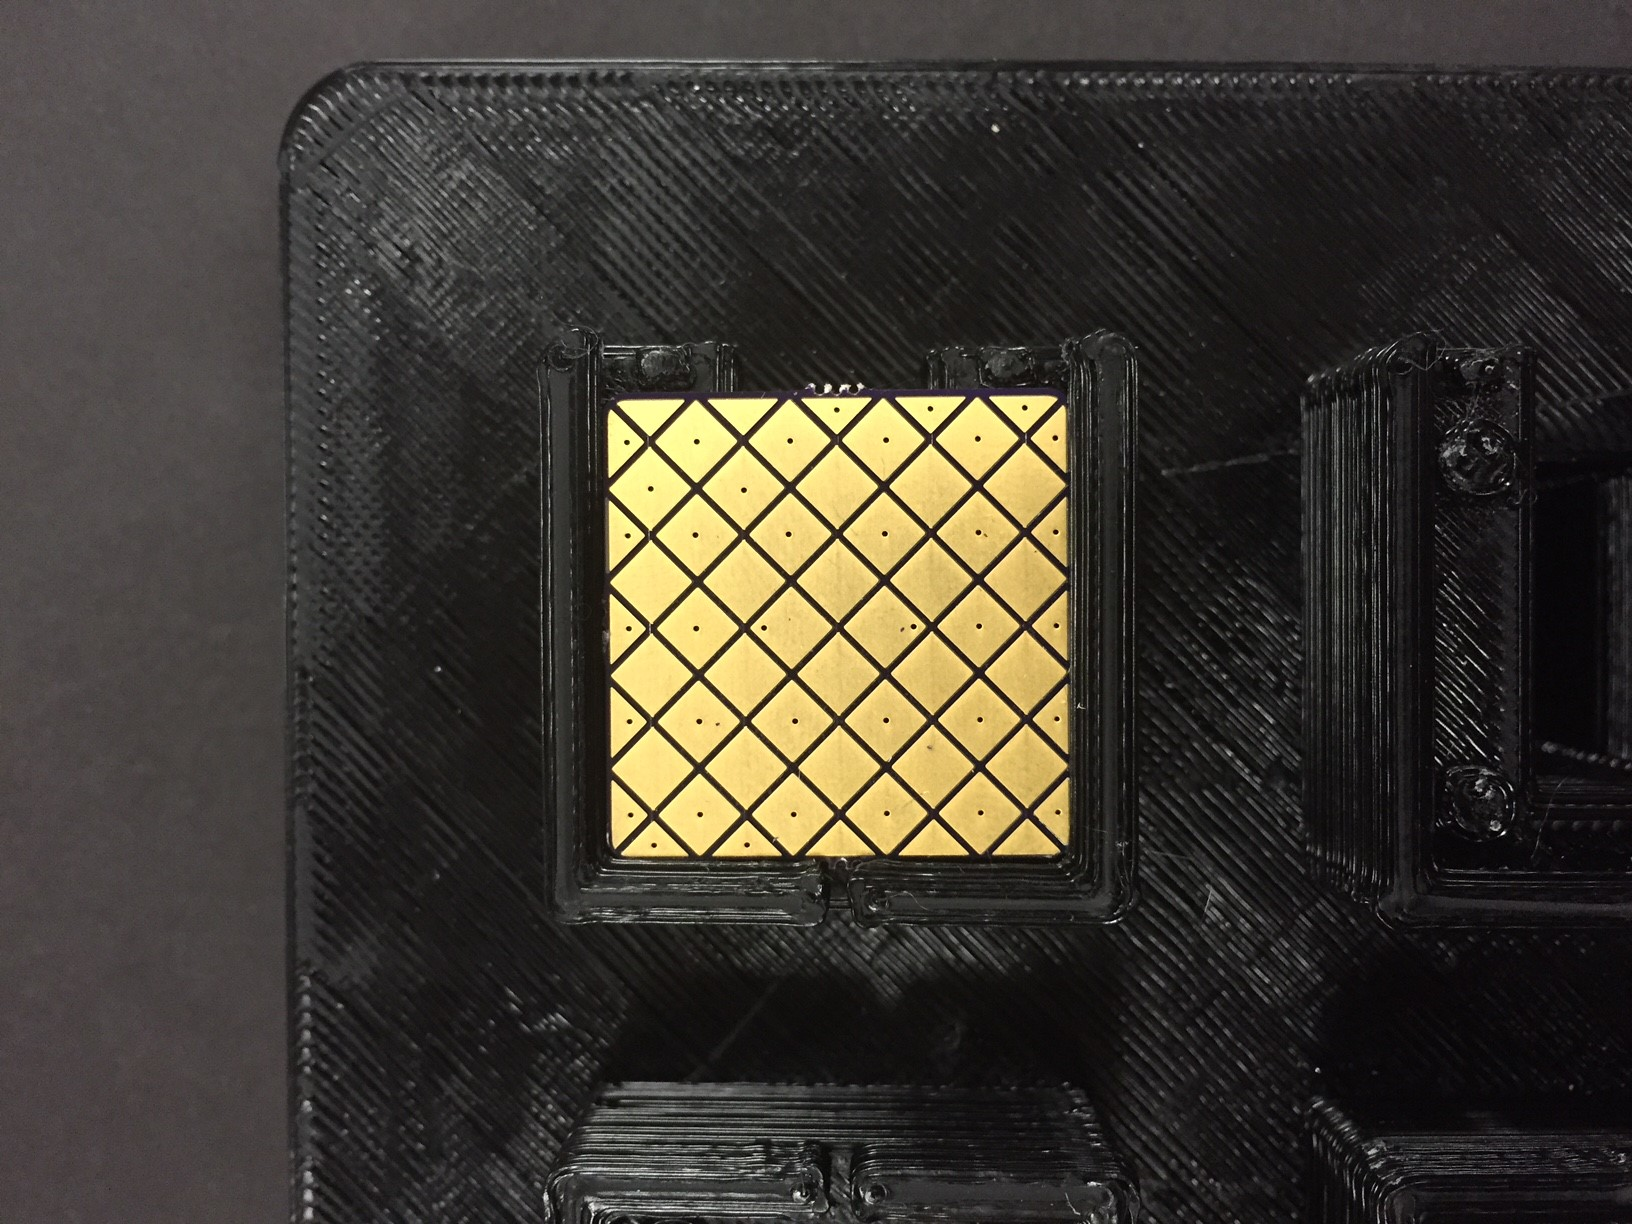
\includegraphics[width=1.25in]{pe_capacitive.jpg}
    \caption{Capacitive touch array button. Each row and column of diamond pads are connected as one electrode each and together can provide location information of where the user presses.}
    \label{fig:pe_capacitive}
\end{figure}

As previously described (Chapter \ref{sec:proto_button_input}), the hand tracker mounted above the panel enables detection of when the user touches a button, ideally without need for a touch sensor.
For this experiment, both sensors were utilized to compare the performance of subjects with both.
The optical tracking button detection uses a simple collision detection box to determine when a subject has pressed a button.
When the finger of the user enters the detection box and remains inside for \SI{50}{\milli\second}, the button press event is activated and recorded.
The purpose of the small delay is to reject false positives if a user moves quickly through the detection box of a button they are not pressing.
The color of the button changes in the virtual world when they enter this detection box to indicate to the user that they are about to register a button press.
For this experiment, the collision detection box was set to extend 0.5 inches inward and outward from the button, including a 0.1-inch tolerance on all dimensions.
\citet{aslandere_virtual_2015} found no significant effect with button selection ability based on changing this volume in a purely virtual environment, so we determined an appropriate size in pilot studies and did not include the size of the detection box as a variable.

\subsection{Experiment Task}

Audio prompts were given through headphones, which indicated the starting pad and panel button goal before each task.
The participants were asked to start with their index finger on the start pad and then target the stated button on the panel.
The use of audio prompts and a delay before starting removes any bias of time to process where they were targeting.
The movement times also do not include the reaction time as they started when subjects lifted their finger from the start pad.

Each participant performed 48 targeting tasks under each of the four different conditions:
\begin{enumerate}
    \item Wearing the HMD, button selection registered by capacitive sensors, panel physically present
    \item Wearing the HMD, button selection registered by hand tracking sensors, panel physically present
    \item Wearing the HMD, button selection registered by hand tracking sensors, panel not physically present
    \item Not wearing the HMD, button selection registered by capacitive sensors, panel physically present
\end{enumerate}
Before each condition the subjects performed one set of 12 trials for familiarization of that particular condition.
This training session was not included in the results.
During the ``no panel'' condition, the hand tracker remained mounted at the same point, but the panel was moved out of the way, such that the subjects were targeting the buttons in the virtual world only.
The button selection in every condition was indicated by a sound played in the headphones when the appropriate sensor measured a button press.
The tasks would time out after 10 seconds.
The task was not repeated for an incorrect button selection or timing out, instead the subject moved on to the next task.
The condition order was randomized for each subject, and the tasks were performed in a pseudo-random order.

\begin{figure}
    \centering
    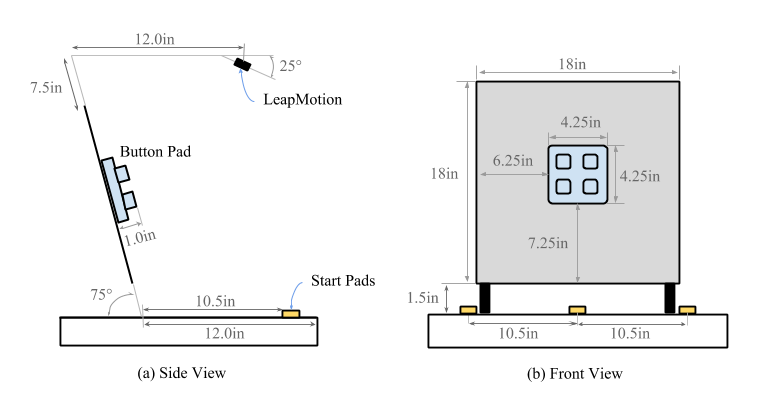
\includegraphics[width=\textwidth]{pe_diagram.png}
    \caption{Diagram of Experiment Setup}
    \label{fig:pe_diagram}
\end{figure}

\begin{figure}
    \centering
    \begin{subfigure}[t]{0.49\linewidth}
        \centering
        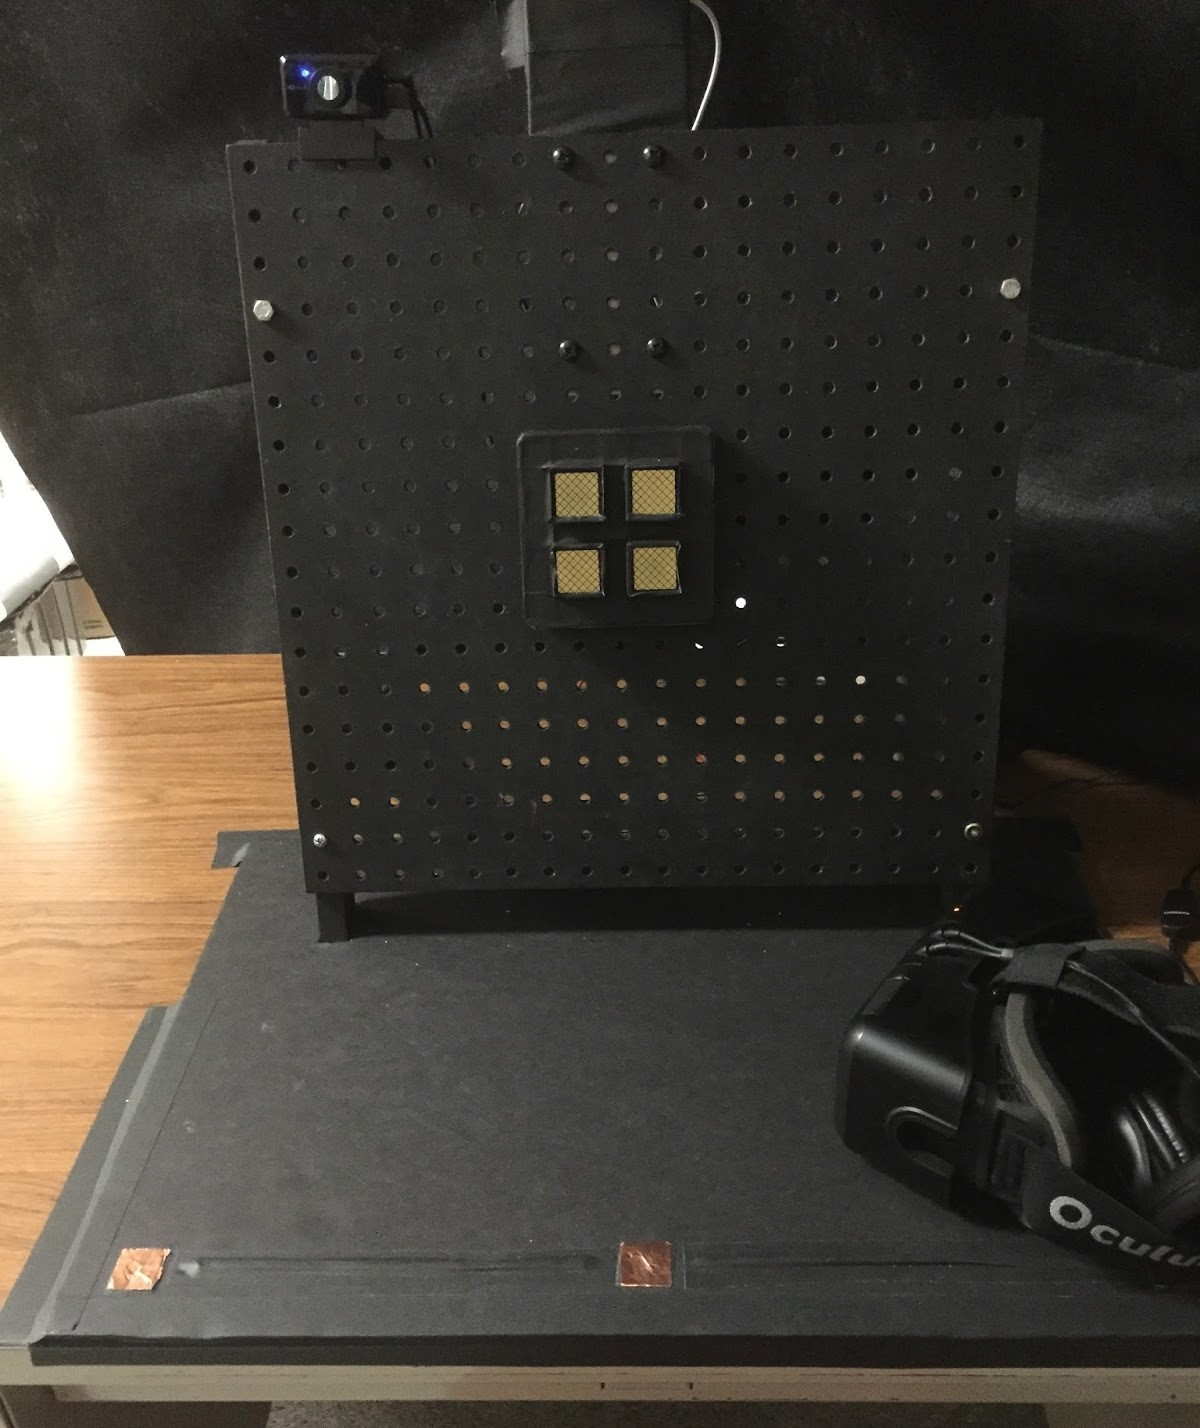
\includegraphics[width=\linewidth]{pointing_real.jpg}
        \caption{Photo of setup in real world.}
        \label{fig:p_setup:real}
    \end{subfigure}
    \begin{subfigure}[t]{0.49\linewidth}
        \centering
        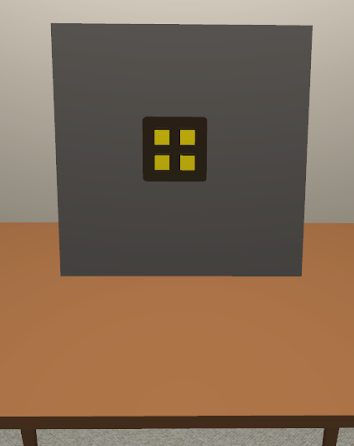
\includegraphics[width=\linewidth]{pointing_virtual.png}
        \caption{View of setup in virtual environment.}
        \label{fig:p_setup:virtual}
    \end{subfigure}
    \caption{Experimental setup and view of virtual environment.}
    \label{fig:p_setup}
\end{figure}

The subjects were all briefed on the technology from a prewritten speech explaining how to activate each of the sensors.
Subjects were instructed to target the center of the correct button, but were given no instructions on speed.
Subjects targeted the button using their index finger of their dominant hand, which was the right hand for all subjects.
No information was given on how to best perform the task or advice on working with the various sensors.

The dependent variables measured were time from starting pad to trial goal button, accuracy as measured on the capacitive touch sensors (for conditions with the panel present), and success rate (selected the correct button within 10 seconds).

%The dependent variables measured were:
%\begin{itemize}
%    \item time from starting pad to trial goal button
%    \item accuracy measured on the capacitive touch sensors (for conditions with the panel present)
%    \item success rate (selected the correct button within 10 seconds)
%\end{itemize}

\subsection{Subjects}
The experiment was performed with 8 subjects, recruited from the university student population, all with no or limited previous exposure to the R3C setup.
All subjects indicated they had either never used a virtual reality headset or briefly tried them once or twice.
Ages ranged from 18-31 with 6 male, 2 female.
They all had correctable vision to 20/20 and none indicated difficulty seeing the image in the virtual reality HMD.
After the experiment, none of the subjects reported symptoms of motion sickness, and only mild eyestrain was reported.
The subjects spent under one hour performing the experiment, with about thirty minutes of virtual reality use.

\section{Results}

The time was recorded for each trial from release of starting pad to the successful button press using the correct button registration.
Trials which timed out or where the incorrect button was targeted were discarded for the time analysis (but not the success rate reported later).
The time for each trial was corrected for the varying distances of the movements by multiplying by the average distance (18.4 in) over the straight-line distance between the start and goal button for that trial (which varied from 15.5in to 20.5in).
The results for each condition are summarized in Table \ref{tab:pe_results}, and Figure \ref{fig:pe_effects} illustrates the three main effects with respect to corrected time.

The significance of the effects were determined using a two sample t-test on the corrected time measure between the appropriate conditions.
The effect of the use of the HMD on corrected movement time was significant ($t(7)=-5.1, p < 0.01$) between condition 1 (HMD, Panel, Capacitive: $M=3.15$ seconds) and 4 (No HMD, Panel, Capacitive: $M=1.57$ seconds).
On average, using the HMD caused the corrected movement time to be 1.58 seconds longer.
The button detection sensor also has a significant effect on corrected time ($t(7)=3.6, p < 0.01$), comparing conditions 1 (HMD, Panel, Capacitive: $M=3.15$ seconds) and 2 (HMD, Panel, Optical: $M=3.78$), but the drop in performance was only 0.63 seconds.
The effect of the panel was found to be not significant ($t(7)=-0.5, p=0.66$) between condition 2 (HMD, Panel, Optical: $M=3.78$) and condition 3 (HMD, No Panel, Optical: $M=3.70$).

\begin{figure}
    \centering
    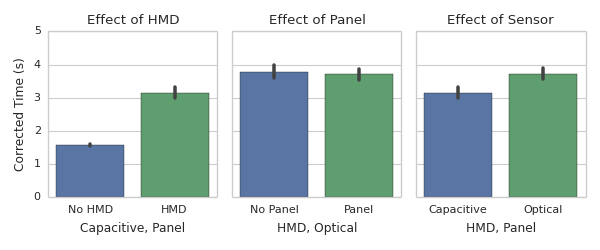
\includegraphics{pointing_effects.png}
    \caption{Major effects studied for corrected time of movement. Effect of HMD and Effect of Sensor are significant effects ($p<0.01$), while Effect of Panel is insignificant.}
    \label{fig:pe_effects}
\end{figure}

\begin{table}
    \centering
    \includetable{pe_results}
    \caption{Mean results across subjects. Distance from center is recorded by capacitive touch sensor. Standard deviations are reported as $\sigma$.}
    \label{tab:pe_results}
\end{table}

The selection of the correct button was performed almost without error, which is a promising result for new users of the system.
There was no significant effect between the different conditions on success rate.
Over 8 subjects and 1517 trials, only 12 trials selected the wrong button and only 12 trials timed out, giving an overall 98.4\% success rate.
Observations made during the experiment suggest that at least some of few incorrect button selections were due to misheard prompts or loss of attention and not due to the system itself.

The accuracy of the button press itself was also measured, and Figure \ref{fig:pe_accuracy} shows the distribution of the locations registered by the capacitive touch sensors.
In the plots, (X,Y) = (0,0) corresponds to the bottom left corner of the button.
The two conditions shown (1 and 4) were the two conditions where capacitive touch registered the button selection.
There is a smaller distribution for the no HMD condition (Figure \ref{fig:pe_accuracy}(b)), but with the HMD (Figure \ref{fig:pe_accuracy}(a)) subjects were still within error to the center of the button.
It should be noted again here that in the HMD condition, subjects had to rely on the virtual hand from the hand tracker for any visual feedback of hand position.

\begin{figure}
    \centering
    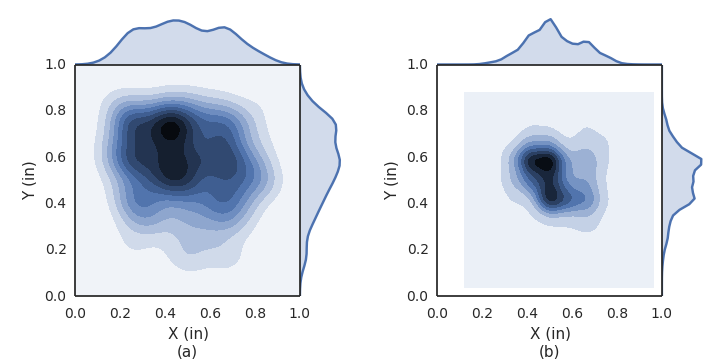
\includegraphics[width=\textwidth]{pe_accuracy.png}
    \caption{Finger press location 2D distribution for (a) HMD, Capacitive, Panel and (b) No HMD, Capacitive, Panel. The distribution is calculated as a Gaussian kernel density estimate. The mean (x, y) location and standard deviation for each is (a) ($0.48\pm0.18, 0.56\pm0.17$) and (b) ($0.52\pm0.12, 0.51\pm0.12$).}
    \label{fig:pe_accuracy}
\end{figure}

A Fitts’ law analysis of the data was not the goal with the experiment design, and since we did not vary the button width a Fitts’ analysis could only be performed with varying distance.
The index of difficulty would only range from 4.0 to 4.5, providing an insufficient range for a proper Fitts’ analysis.
Including extra parameters for the 3D nature of the task \citep{murata_extending_2001, cha_extended_2013} did not improve the fit, especially considering the symmetry of the setup.
Furthermore, the time recorded of the tasks were typically more than in a Fitts' task, since many subjects spent time honing based on the accuracy instructions.

%The hand tracker was recording the trajectory in every condition.
%Figure 7 shows representative trajectories of a movement from the left start pad to the top right panel button.
%The button area is shown as a blue box as well on the plots.
%Figure 7(a) shows the trajectory of every subject for HMD, Optical, Panel condition.
%Figure 7(b) focuses on one subject where each line corresponds to each condition.
%This shows a sample of the variation of their trajectory for each condition.
%The plots are both centered at the bottom left corner of the goal button, the z-axis is perpendicular to the button, the y-axis is pointing up from the desk along the panel, and the x-axis is pointed to the right.

%\begin{figure}
%    \centering
%    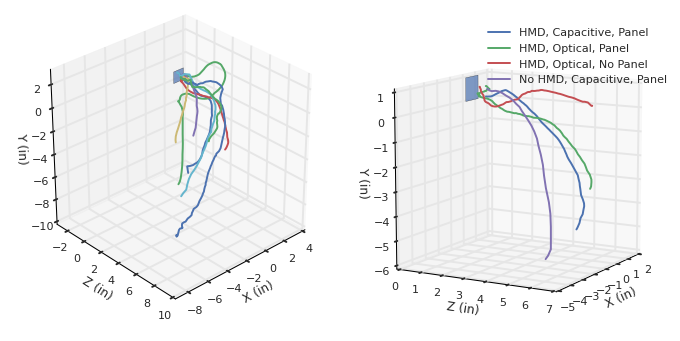
\includegraphics{pe_trajectory.png}
%    \caption{Trajectories of movement for a single trial from left starting pad to top right panel button, for (a) all subjects in HMD, Optical, Panel condition, and (b) one subject, all conditions.}
%    \label{fig:pe_trajectory}
%\end{figure}

\section{Discussion}

The start pads and hand tracker were located relative to each other in such a way that the hand would not be in view of the tracker at the beginning of the task, thus the user would have to wait for the hand tracker to acquire the hand when in view.
This meant for the trials using the HMD the subject would typically have an open loop (blind) ballistic phase followed by the closed loop homing phase once the virtual hand appeared in the virtual world.
Across subjects for all HMD conditions, this hand acquisition by the tracker took on average \SI{660}{\milli\second} ($\sigma = \SI{649}{\milli\second}$) from leaving the start pad.
An expert user who performed the experiment was able to get the hand to appear in the tracker in \SI{330}{\milli\second} ($\sigma = \SI{133}{\milli\second}$) on average.
This could indicate that training on how to get the best hand tracker performance could improve results.
The same expert also only experienced a \SI{416}{\milli\second} slowdown between using the HMD and not using the HMD (conditions 1 and 4), compared to the \SI{1580}{\milli\second} slowdown measured across the 8 new subjects.

We had originally hypothesized that having the panel would improve the selection performance of the button, but for this task it had no effect.
There are two possible contributing factors that reduced the effect of the panel on the performance of the subjects.
First, the subjects were instructed to target the center of the button.
Some subjects spent time ensuring they were centered over the button before they even entered the zone in front of the button, thus eliminating the need for the panel to provide location.
Secondly, this task was a discrete pointing task, where the subject would `reset' to the starting position on the desk between each movement.
It is possible that the panel being in position would help the subject build a better sense of the relative locations of the buttons when moving between buttons on the panel (a serial task).
%awk af
For this task the passive haptic may not provide a benefit when they only target one button on the panel before returning to the start pads.
It is also possible that while the panel did not improve targeting performance in this task, it may provide a benefit to the subjective feeling of presence in the virtual world, which may be beneficial in a more demanding situation with multiple tasks.

Another variable that was not measured was fatigue.
Having the panel as a backstop may decrease the amount of fatigue for a repeated targeting task, as floating the arm in free space to target a button in a purely virtual environment with no panel can cause a buildup of arm fatigue.
If the virtual world and physical world are correctly aligned, then the finger can momentarily rest on the button while the hand tracker works to detect a button press.

Overall, the lack of an effect of the panel could also be interpreted as a positive result.
As discussed before, a significant problem we've been working on is the improvement of tracking performance when the hand nears the panel.
The results indicate that this problem has been mitigated at least as much to provide performance on par with the purely virtual world.

\section{Conclusion}

%\begin{figure}
%    \centering
%    \includegraphics{pe_future.png}
%    \caption{Screenshot from a current demo: User is controlling an external camera on the International Space Station from the cupola.}
%    \label{fig:pe_future}
%\end{figure}

We have shown that new users can accurately select buttons in a simple targeting task in our system.
All of our independent variables showed no significance on correct button selection.
The use of the head-mounted display to provide visuals of hand position provides a small time penalty in button selection.
The use of the physical panel provided no significant effect in time compared to having the subjects target purely virtual buttons.
Our optical tracking algorithm had a slight negative effect in time compared to using the capacitive touch sensors.
